\chapter{Evaluation}

This chapter will explore the testing process of the application's frontend and backend, followed by the evaluation of the MLLM and ending with brief analysis of stakeholder feedback.

\section{Frontend Testing}

Frontend testing was conducted manually due the time constraints, component complexity and lack of experience with automated testing frameworks. To ensure consistency in the testing procedure, structured test cases was created for most components. These test cases used the Gherkin syntax, which follows the Given-When-Then format \parencite{gherkin}. 

An example of test cases for the share link record selection functionality is shown below. The testing outcomes can be viewed in figures~\ref{fig:test1},~\ref{fig:test2} and~\ref{fig:test3}, which demonstrate the implementation of the selection behaviour.

To ensure an even coverage of all implemented components, a site map was created to document all pages, components and their relationships. This figure provided a high-level system overview and aided the testing progress tracking. The site map can be seen in figure~\ref{fig:sitemap}.

\clearpage

\begin{lstlisting}[language=Gherkin, caption=Test cases for selecting records to be shared in a share link]
    Feature: Record selection for share link

    Scenario: User selects all record types to be shared
        Given the user is on the share link page
        When the user selects the top checkbox to select all record types
        Then all record types should be selected for sharing
        And the all children checkboxes should be selected as well 
    
    Scenario: User selects specific record types to be shared
        Given the user is on the share link page
        When the user selects a specific record type to be shared
        Then only the selected record types should be selected for sharing
        And the respective children checkboxes should all be selected as well

    Scenario: User selects specific children records to be shared
        Given the user is on the share link page
        When the user selects specific children records to be shared
        Then only the selected children records should be selected for sharing
        And the respective parent checkbox should not be selected
        And the top child checkbox should not be selected
\end{lstlisting}

\begin{figure}[htbp]
    \centering
    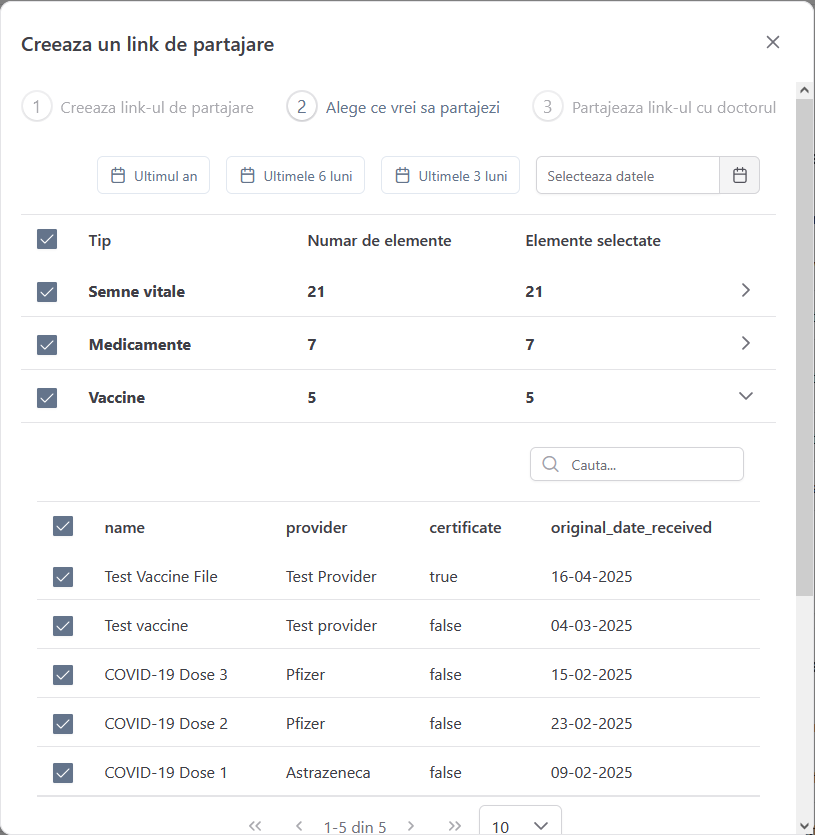
\includegraphics[width=\textwidth]{TestCase_All.png}
    \caption{Test Scenario \#1}\label{fig:test1}
\end{figure}

\begin{figure}[htbp]
    \centering
    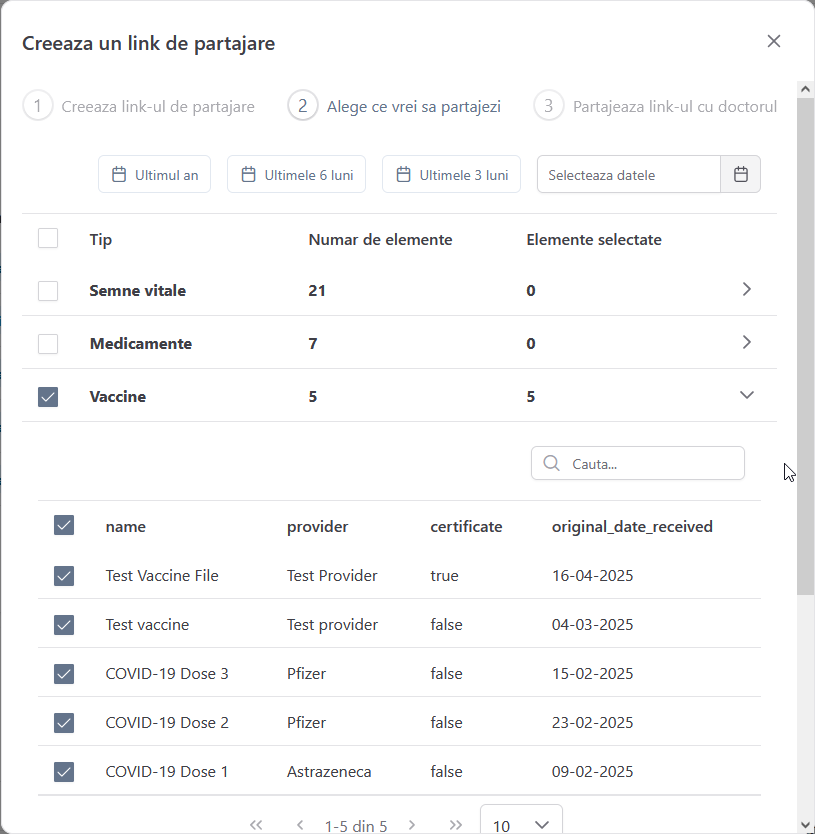
\includegraphics[width=\textwidth]{TestCase_One.png}
    \caption{Test Scenario \#2}\label{fig:test2}
\end{figure}

\begin{figure}[htbp]
    \centering
    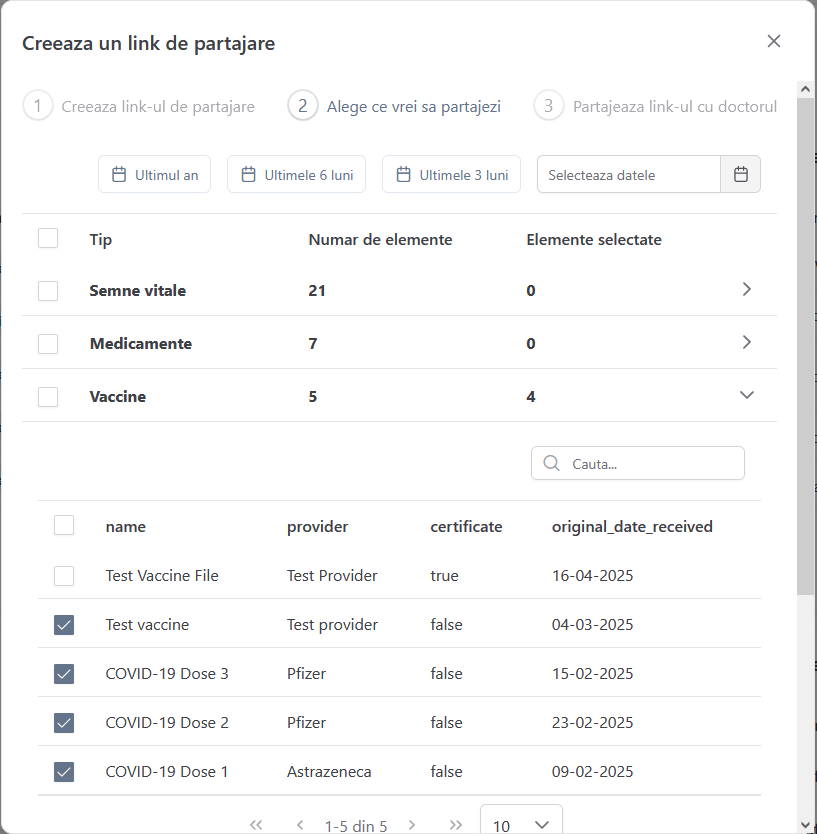
\includegraphics[width=\textwidth]{TestCase_SomeChild.png}
    \caption{Test Scenario \#3}\label{fig:test3}
\end{figure}

\begin{figure}[htbp]
    \centering
    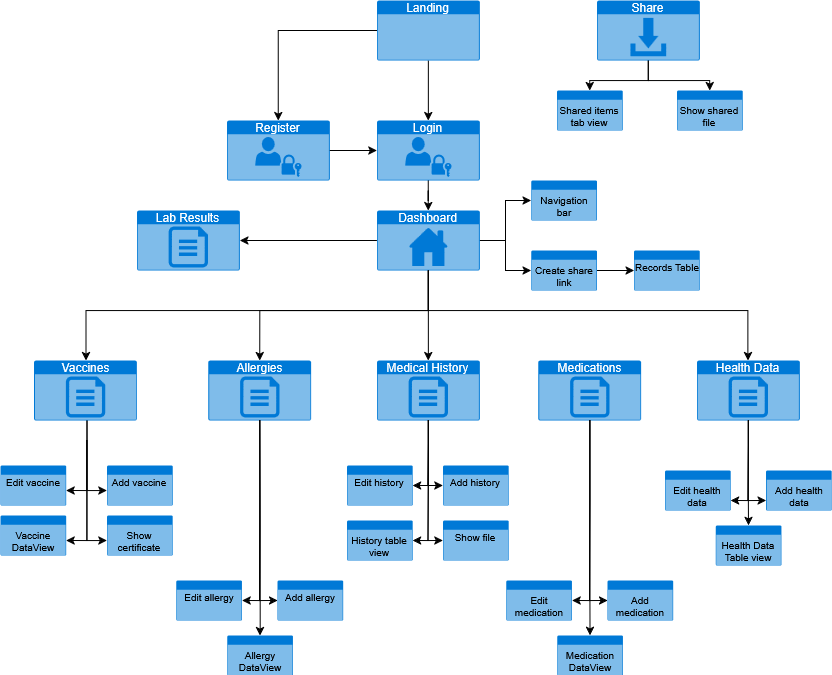
\includegraphics[width=\textwidth]{SiteMap.png}
    \caption{PHR System Site Map}\label{fig:sitemap}
\end{figure}

\FloatBarrier{}

\section{Backend Testing}

Backend testing was conducted through two approaches: indirect testing, done in parellel with the frontend, and direct testing by using Postman for the API endpoints. The backend's reduced complexity, compared to the frontend, allowed for a more straightforward testing process. The backend functionality was often tested in conjunction with the frontend, as the frontend components relied on the backend to function correctly. This meant that many of the test cases were already covered during the frontend testing process.

To ensure correct endpoint behaviour and functionality, the endpoints were additionally tested using Postman, without relying on the frontend components. The following example illustrates the testing of the share link validation endpoint:

\begin{lstlisting}[language=Python, caption=Example endpoint for checking a share link for expiration time]
    @router.get("/share/{share_code}", status_code=status.HTTP_200_OK)
@limiter.limit("5/minute")
async def check_share_token(
    request: Request,
    share_code: str,
    session: Session = Depends(get_session)):
    share_token = session.exec(select(ShareToken).where(ShareToken.share_code == share_code)).first()
    
    if not share_token:
        raise HTTPException(status_code=status.HTTP_404_NOT_FOUND, detail="Share token not found")
    
    if share_token.expiration_time < datetime.now():
        raise HTTPException(status_code=status.HTTP_410_GONE, detail="Share token has expired")
    
    return {"valid": True}
\end{lstlisting}

The endpoint above validated three scenarios: invalid, expired and valid share tokens. Each scenario would be tested individually for the correct status code and response message using Postman, as can seen in figures~\ref{fig:postman1},~\ref{fig:postman2} and~\ref{fig:postman3}.

\begin{figure}[htbp]
    \centering
    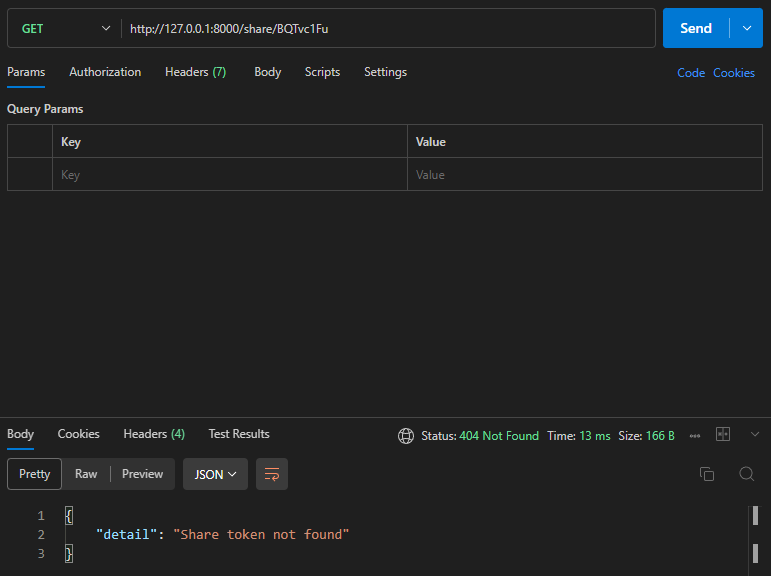
\includegraphics[width=\textwidth]{PostmanNotFound.png}
    \caption{Postman test --- share token not found}\label{fig:postman1}
\end{figure}

\begin{figure}[htbp]
    \centering
    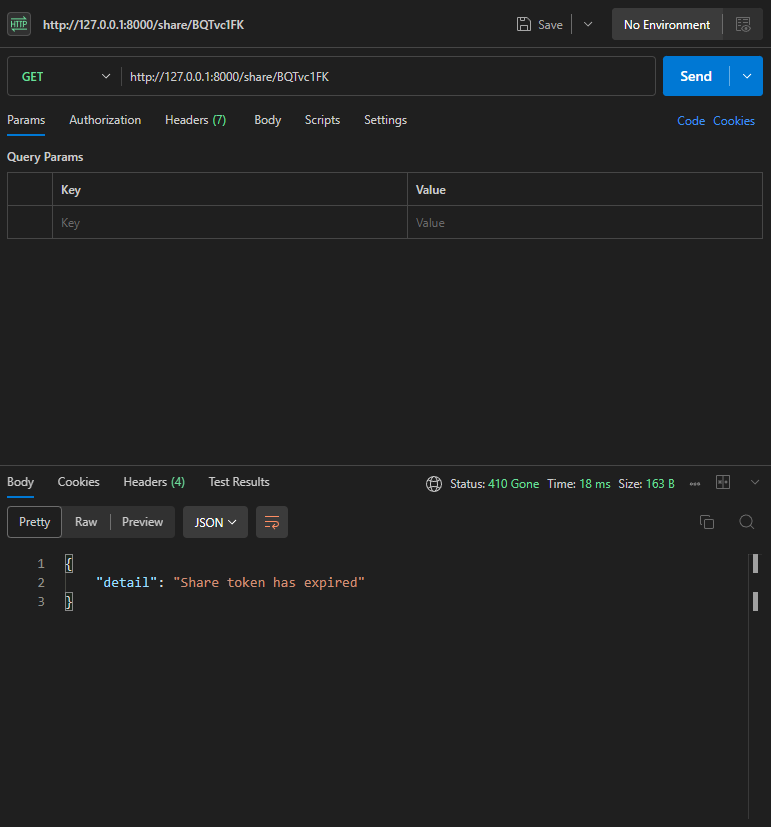
\includegraphics[width=\textwidth]{PostmanExpired.png}
    \caption{Postman test --- share token expired}\label{fig:postman2}
\end{figure}

\begin{figure}[htbp]
    \centering
    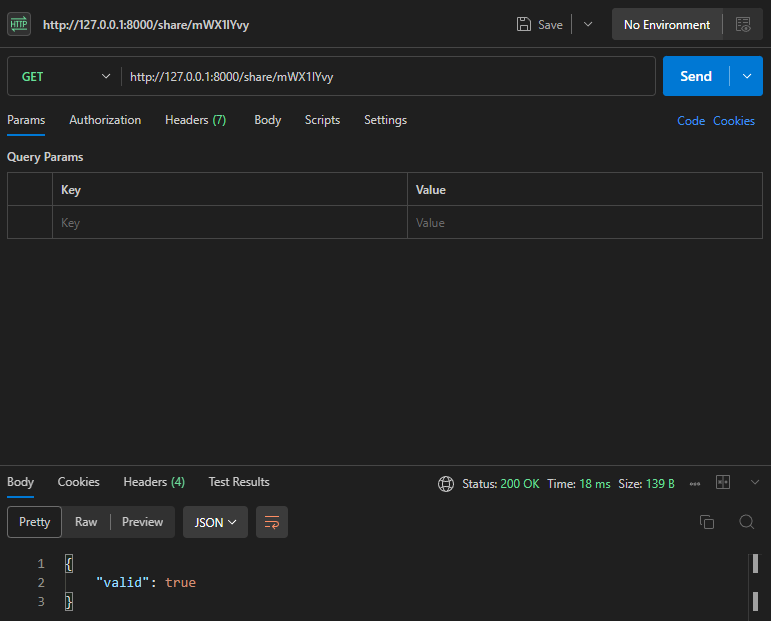
\includegraphics[width=\textwidth]{PostmanOK.png}
    \caption{Postman test --- share token valid}\label{fig:postman3}
\end{figure}

\FloatBarrier{}

\section{LLM Evaluation}

Gemini 2.0 Flash was selected as the MLLM that powers the lab results extraction feature based on its generous free tier allocation (15 requests/minute with 1,000,000 tokens/minute), robust multimodal capabilities and competitive performance. As of writing this section, this model ranked among the top 10 models on the Chatbot Arena leaderboard for both language and vision tasks created by~\cite{chatbotarena}, showcasing its strong performance relative to similar models. As described by its authors, the leaderboard is an `open platform for crowdsourced AI benchmarking', which generates live leaderboards based on user feedback from comparing responses from different models.

Further model evaluation on its lab result extraction capabilities included testing the model's performance on a set of documents from different healthcare institutions in Moldova. Three distinct documents were used for the evaluation --- 2 from private lab networks and 1 from a private hospital. These institutions were chosen for their popularity and wide network of locations across the country \parencite{alfalab, synevo, medpark}. The anonymised documents, alongside their extracted results, can be seen in figures~\ref{fig:synevo},~\ref{fig:alfalab} and~\ref{fig:medpark}.

\begin{figure}[ht]
    \centering
    \subfloat[Lab document]{%
        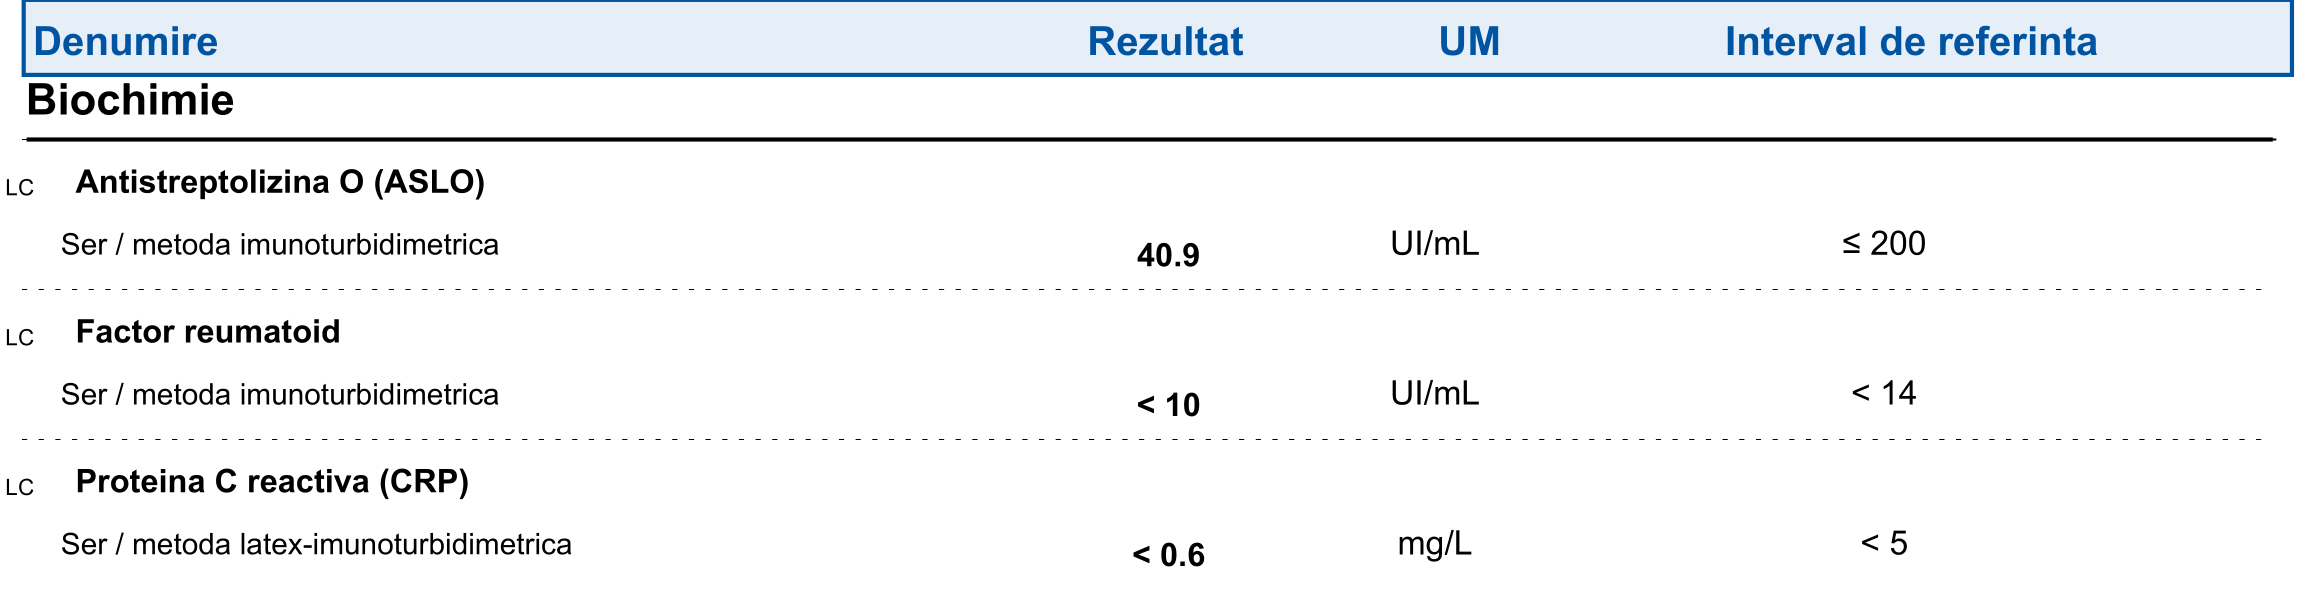
\includegraphics[width=0.9\textwidth]{Synevo_edited.png}%
    }
    \\[\baselineskip]
    \subfloat[Extraction result]{%
        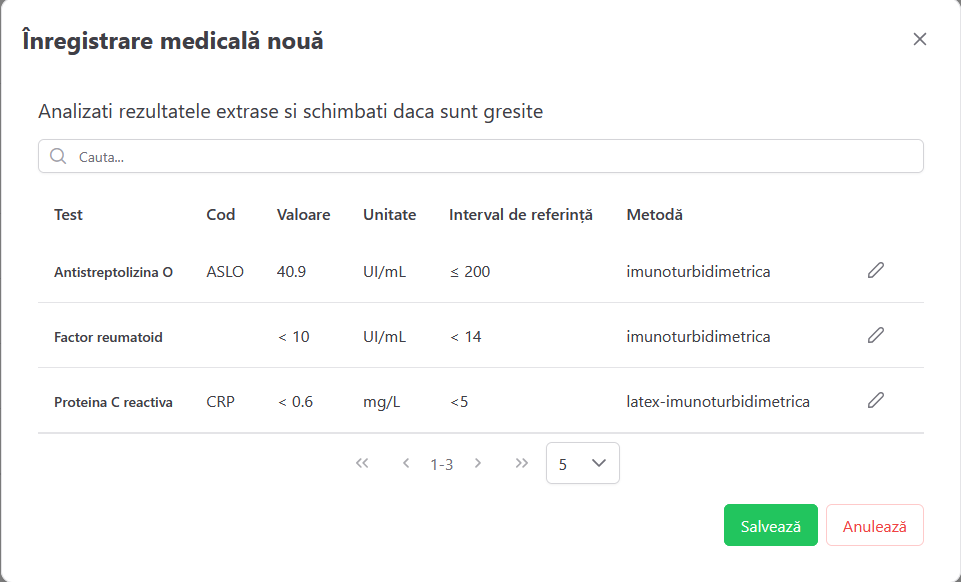
\includegraphics[width=0.9\textwidth]{Synevo_result.png}%
    }
    \caption{Synevo extraction results}\label{fig:synevo}
\end{figure}

\begin{figure}[ht]
    \centering
    \subfloat[Lab document]{%
        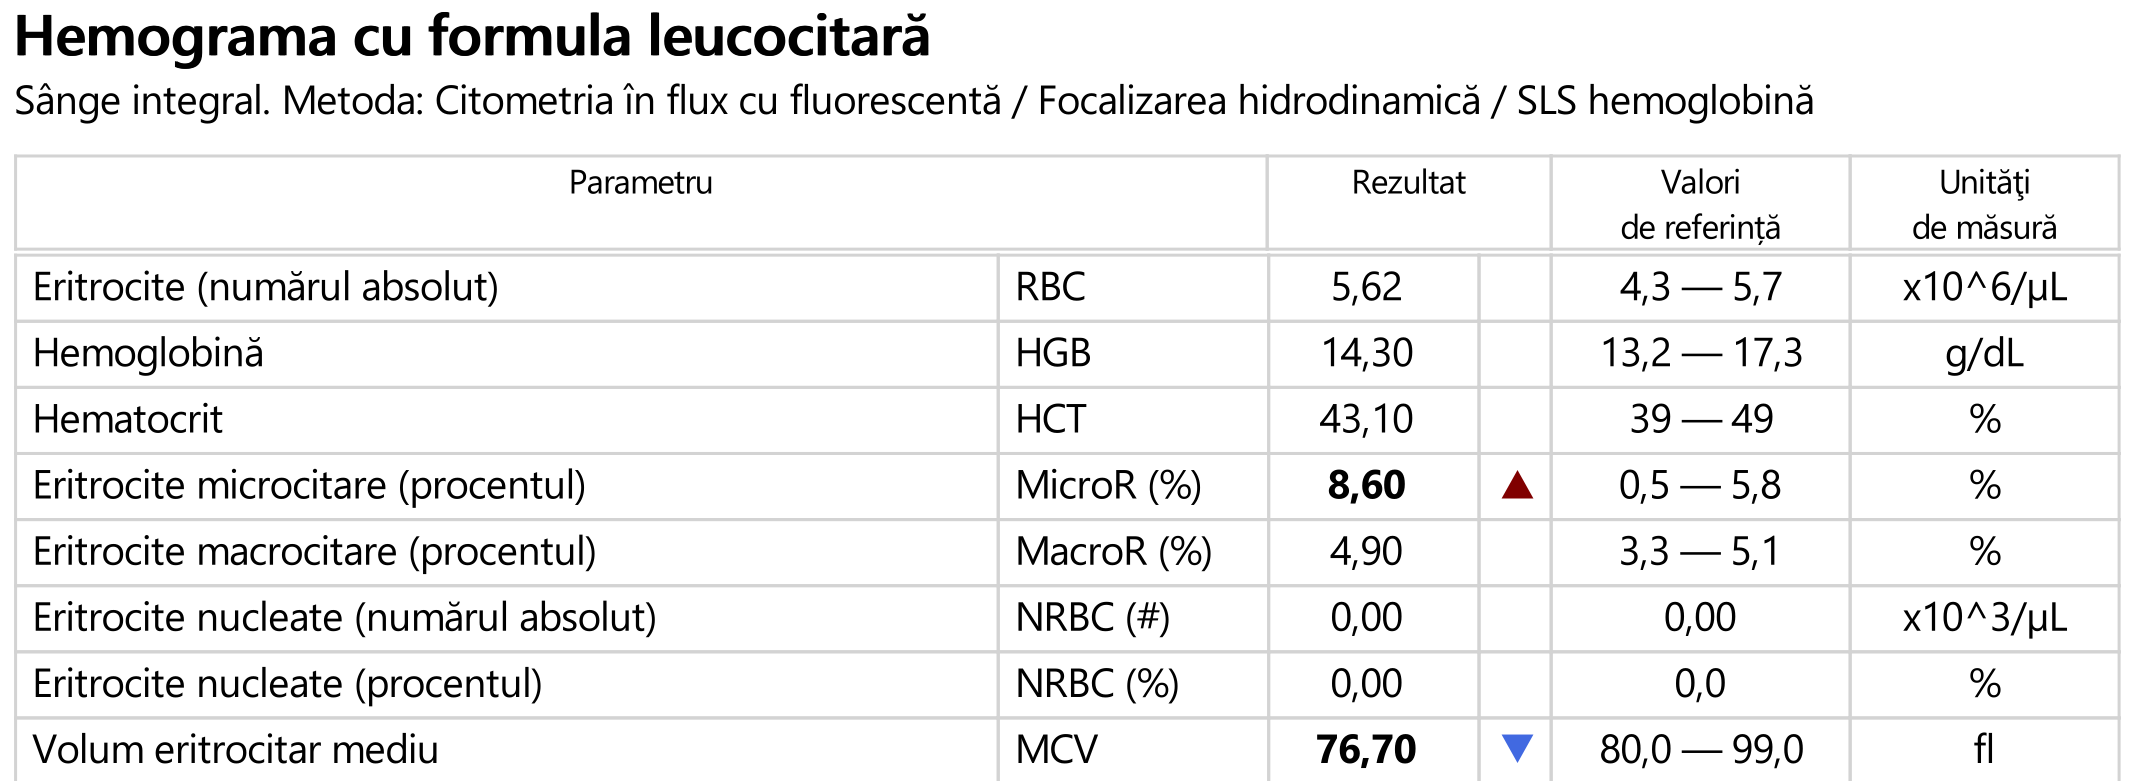
\includegraphics[width=0.9\textwidth]{Alfalab_edited.png}%
    }
    \\[\baselineskip]
    \subfloat[Extraction result]{%
        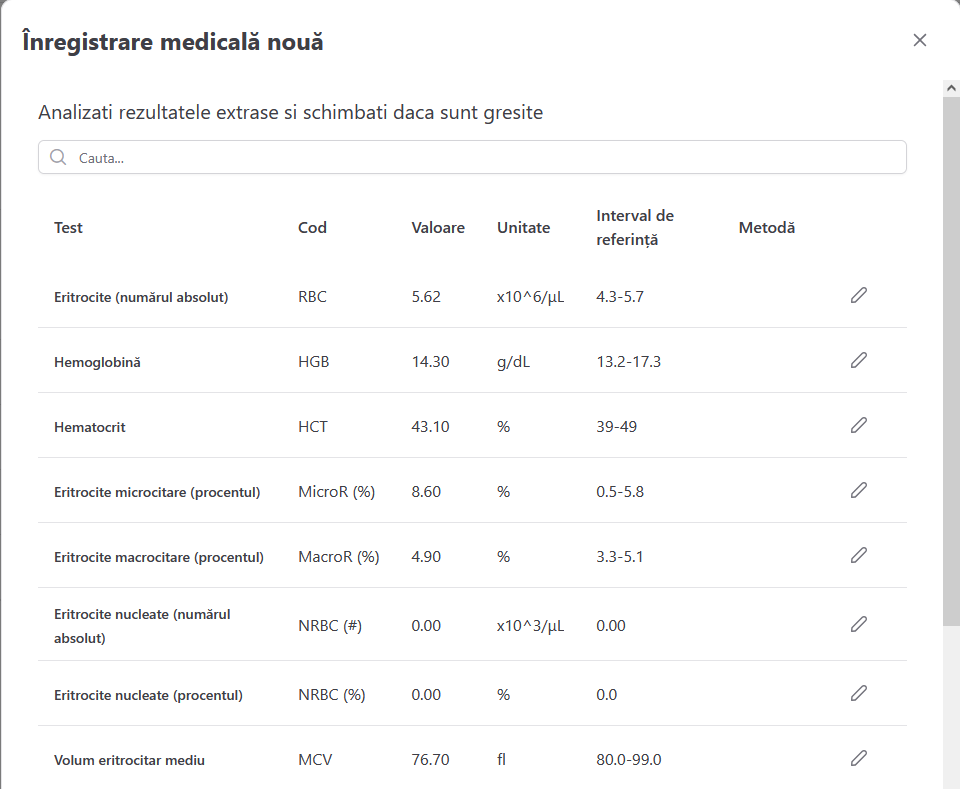
\includegraphics[width=0.9\textwidth]{Alfalab_result.png}%
    }
    \caption{Alfalab extraction results}\label{fig:alfalab}
\end{figure}

\begin{figure}[ht]
    \centering
    \subfloat[Lab document]{%
        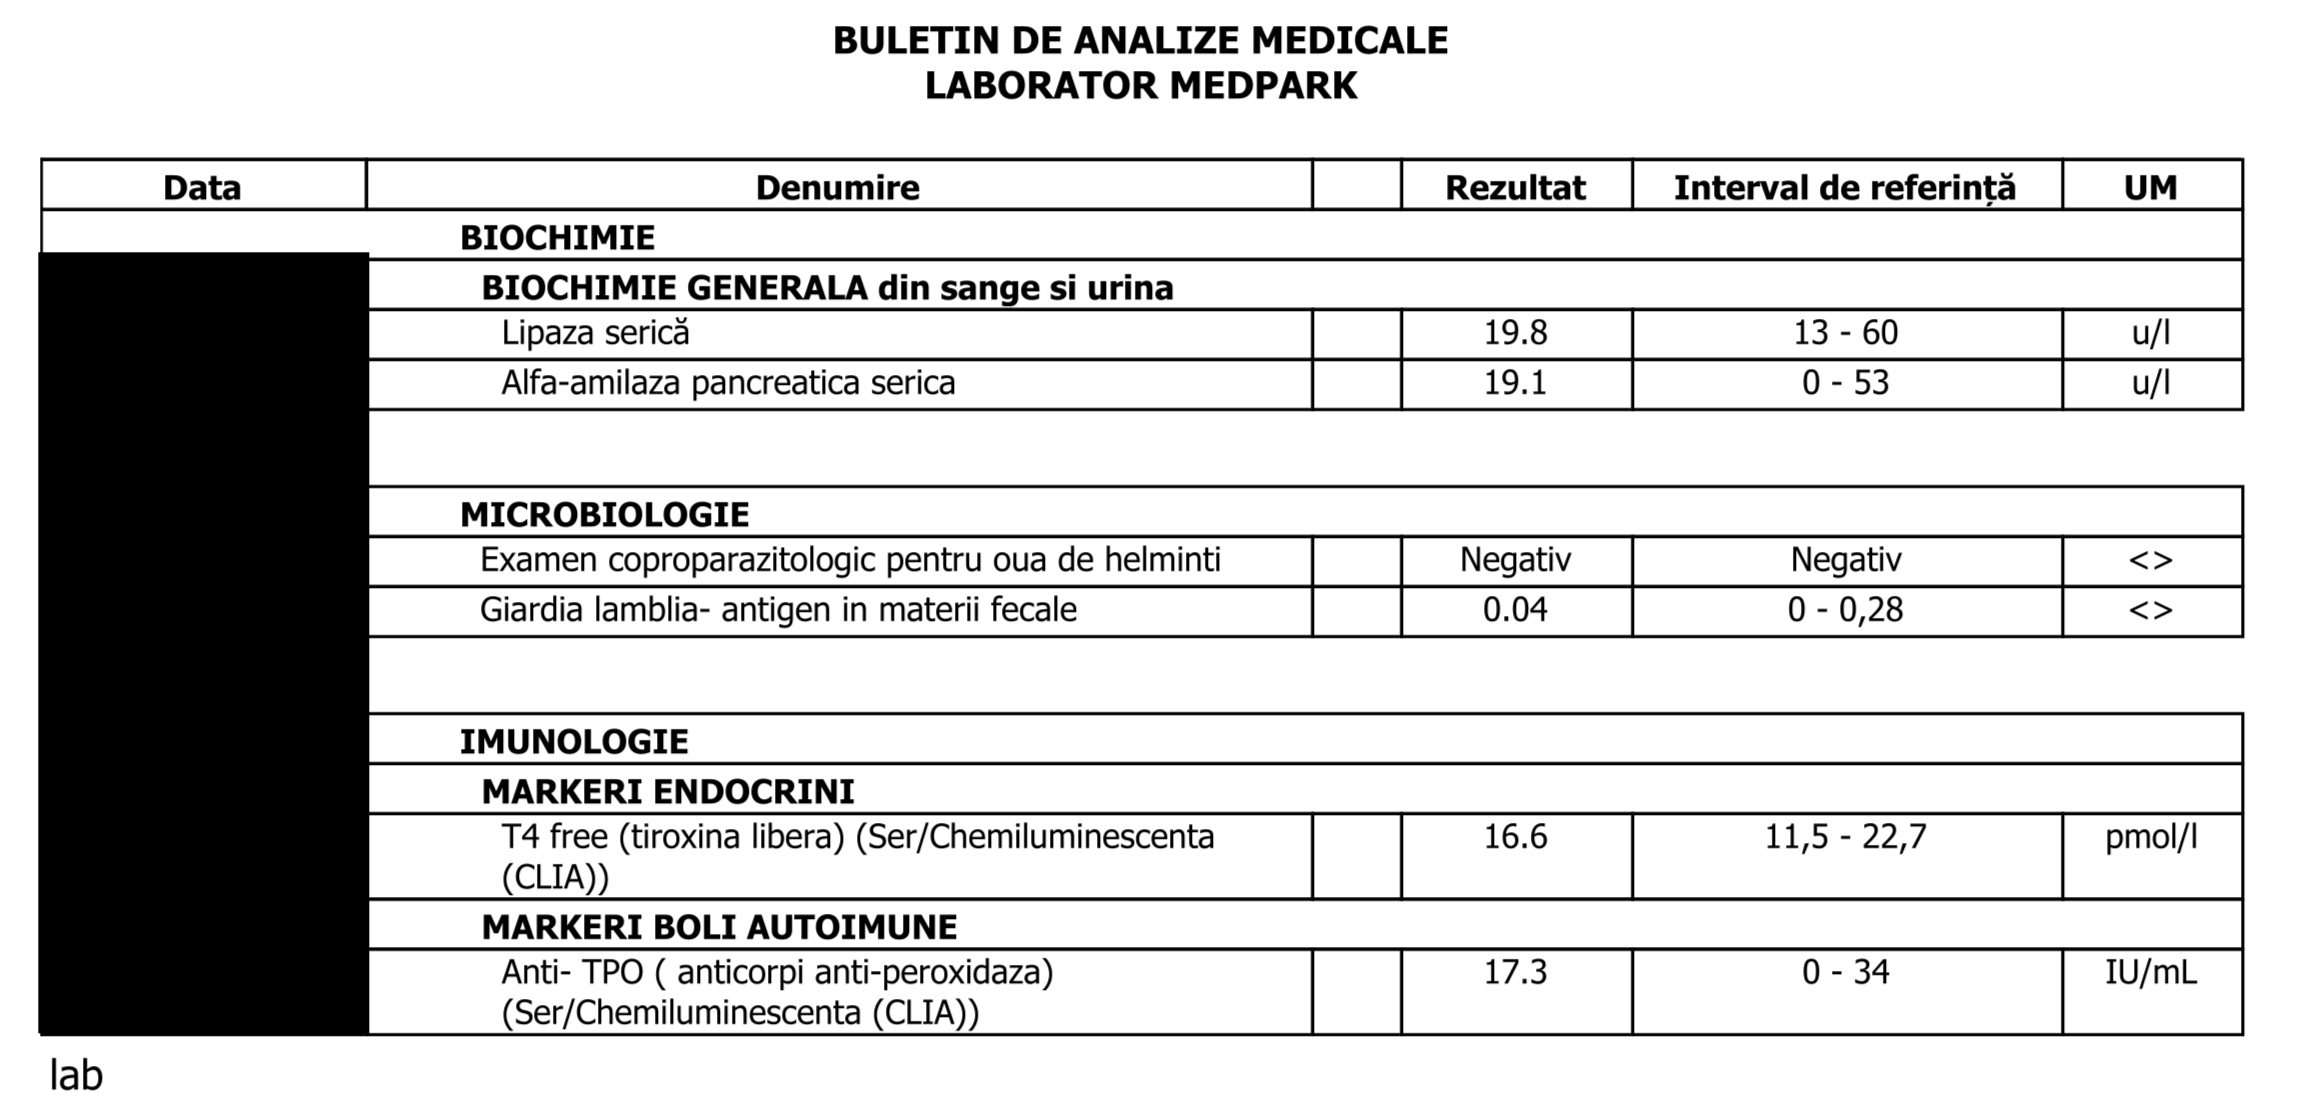
\includegraphics[width=0.9\textwidth]{Medpark_edited.png}%
    }
    \\[\baselineskip]
    \subfloat[Extraction result]{%
        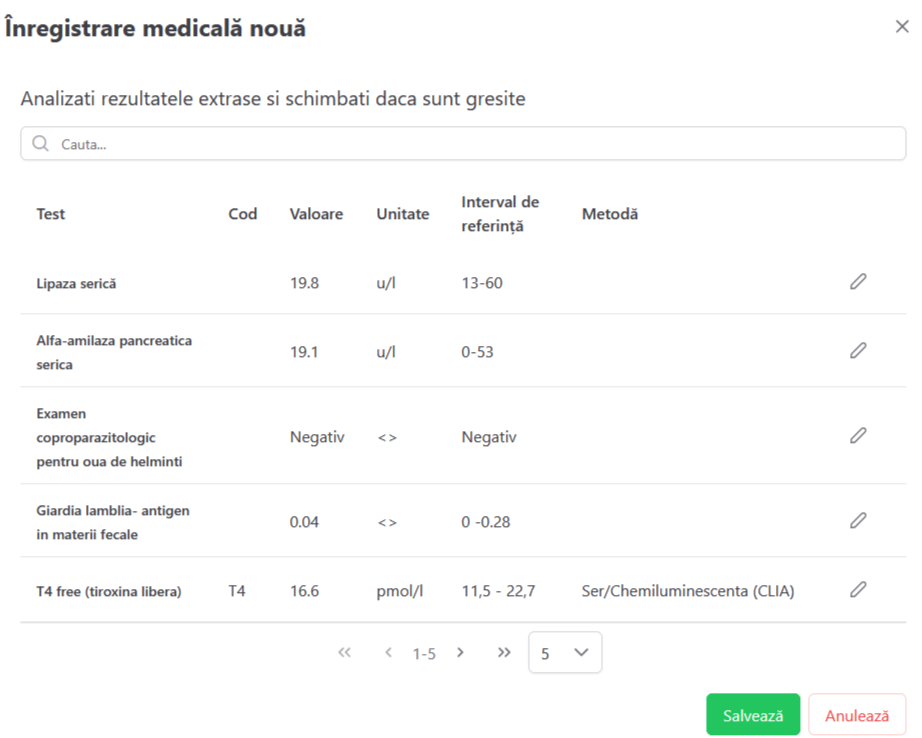
\includegraphics[width=0.9\textwidth]{Medpark_result.png}%
    }
    \caption{Medpark extraction results}\label{fig:medpark}
\end{figure}

In conclusion, the evaluation demonstrated Gemini 2.0 Flash's strong quality and consistent performance across different documents, succesfully extracting test names, codes, values, units, reference ranges and methods. By using a single prompt for all documents, the model was able to deliver consistent results, regardless of the document's format or content, validating its selection for the task at hand.

\section{Stakeholder feedback}

The system evaluation process concluded with final stakeholder feedback, which was collected through live demo sessions via virtual meetings. Stakeholders were encouraged to provide their feedback in a free format, without any structured questionnaire or formal feedback collection process, allowing for a natural and open discussion. Anonymised excerpts can be seen below, with full feedback available in appendix~\ref{sec:full_feedback}.


Feedback 1, from a medical doctor specialised in digital healthcare applications:

\begin{quotation}
    `I appreciated the concept of the project and the way all essential components of a Personal Health Record were integrated: general, clinical, and paraclinical data, consultations, physician access, and data security. The platform is strongly patient-centered, enhancing access to personal medical data and significantly contributing to patient empowerment \textellipsis{} From my perspective as a medical doctor specialized in public health and an expert in digital transformation of healthcare, I see great potential in this project and I am committed to offering the necessary support for its further development'
\end{quotation}

Feedback 2, from a patient and healthcare user:

\begin{quotation}
    `I was really impressioned with the application on the digital health records book you have developed and presented to me. As a BA you have managed to capture the most important needs and then translated them into useful features included in the solution developed \textellipsis{} By developing this solution you have given a new opportunity to Moldova to make one big step forward to the digitisation, and hope it will be largely used by moldovans as the country offers them also other related nice opportunities like high speed internet access and good coverage by 5G network'
\end{quotation}